\documentclass{article}

\usepackage[total={7in,10in}]{geometry}

% basic
\usepackage{comment}
\makeatletter
\@ifclassloaded{revtex4-2}{}{
	\@ifclassloaded{standalone}{}{
		\@ifclassloaded{beamer}{}{
			\usepackage{geometry} % only use geometry outside of RevTeX and TeXit
		}
	}
}
\makeatother
\usepackage{microtype}
\usepackage[dvipsnames]{xcolor}
\usepackage{titlesec}

% programmability
\usepackage{xparse}
\usepackage{xtemplate}
\usepackage{ifthen}
\usepackage{xintexpr}
\usepackage{mathcommand}

% Support for CJK characters
\ifthenelse{\equal{\meaning\pdftexbanner}{\meaning\someundefinednonsense}}{
	\ifthenelse{\equal{\meaning\luatexbanner}{\meaning\someundefinednonsense}}{
		% xelatex
		\usepackage[UTF8]{ctex}
	}{
		% lualatex
	}
}{
	% pdflatex
	\usepackage{CJKutf8}
	\AddToHook{begindocument/end}{\CJK{UTF8}{gbsn}}
	\AddToHook{enddocument}{\endCJK}
}

% fonts
\usepackage{amsfonts} % for \mathbb, \mathfrak
\usepackage{mathrsfs} % for \mathscr
\usepackage{bm}
\usepackage{upgreek}

\newcommand{\mbb}[1]{\mathbb{#1}}
\newcommand{\mfk}[1]{\mathfrak{#1}}
\newcommand{\mrm}[1]{\mathrm{#1}}
\newcommand{\trm}[1]{\textrm{#1}}
\newcommand{\mbf}[1]{\mathbf{#1}}
\newcommand{\tbf}[1]{\textbf{#1}}
%\newcommand{\mit}[1]{\mathit{#1}}
\newcommand{\msf}[1]{\mathsf{#1}}
\newcommand{\mcal}[1]{\mathcal{#1}}
\newcommand{\mscr}[1]{\mathscr{#1}}
%\newcommand{\mtt}[1]{\mathtt{#1}}
\newcommand{\tit}[1]{\textit{#1}}
\newcommand{\ttt}[1]{\texttt{#1}}
\newcommand{\bs}[1]{\boldsymbol{#1}}

% basic utilities
\usepackage{mathtools}
\usepackage{amsthm}
\usepackage{verbatim}
\usepackage{lipsum}

% extensions
\usepackage{cancel} % \cancel
\usepackage{tensor} % \tensor, \indices
\usepackage{fixdif} % \d
\usepackage[shortlabels]{enumitem} % options to enumerate and itemize environments
\usepackage{dcolumn} % align numbers by decimal point in tabular
\usepackage{hyperref} % \url, \href, and add hyperlinks to crossrefs
\usepackage{scalerel} % \scalerel, \stretchrel, \scaleto, \stretchto
\usepackage[notquote]{hanging} % \hangpara
\usepackage{chngcntr} % \counterwithin, \counterwithout
\usepackage{slashed} % \slashed

\makeatletter
\@ifclassloaded{beamer}{
	% https://tex.stackexchange.com/a/24491
	\setitemize{label=\usebeamerfont*{itemize item}%
	\usebeamercolor[fg]{itemize item}
	\usebeamertemplate{itemize item}}
}{}
\makeatother

% beamer style
\makeatletter
\@ifclassloaded{beamer}{
	\usetheme{Boadilla}
	\usefonttheme{serif}
	\setbeamertemplate{footline}{% https://tex.stackexchange.com/a/67000
		\leavevmode%
		\hbox{%
			\begin{beamercolorbox}[wd=.2\paperwidth,ht=2.25ex,dp=1ex,center]{author in head/foot}%
				\usebeamerfont{author in head/foot}\insertshortauthor
			\end{beamercolorbox}%
			\begin{beamercolorbox}[wd=.8\paperwidth,ht=2.25ex,dp=1ex,center]{title in head/foot}%
				\usebeamerfont{title in head/foot}\insertshorttitle\hspace*{3em}
				\insertframenumber{} / \inserttotalframenumber\hspace*{1ex}
			\end{beamercolorbox}
		}%
		\vskip0pt%
	}
}{}

% floats
\usepackage{listings}
\lstdefinestyle{mystyle}{
	basicstyle=\ttfamily\scriptsize,
	tabsize=2,
	showspaces=false,
	showstringspaces=false,
	extendedchars=true
}
\lstset{style=mystyle}

\makeatletter
\@ifclassloaded{revtex4-2}{
	% https://tex.stackexchange.com/a/597712
	\usepackage[caption=false]{subfig}
	\usepackage{ragged2e}
	\DeclareCaptionJustification{justified}{\justifying}
}{
	\usepackage{caption} % not compatible with RevTeX
	\usepackage{subfig}
}
\makeatother

\usepackage{graphicx} % \includegraphics
\usepackage{booktabs} % \toprule, \midrule, \bottomrule
\setlength{\tabcolsep}{12pt}

% fancy tools
\usepackage[version=4]{mhchem}
\usepackage{chemfig}
\usepackage{chemmacros}

\usepackage{physics2}
\usephysicsmodule[empty={}]{diagmat}
\usephysicsmodule{doubleprod}
\usephysicsmodule{xmat}

\usepackage[separate-uncertainty=true,multi-part-units=single]{siunitx}
\sisetup{range-phrase=--, range-units=single} % use -- for ranges, unit appears only once
\catcode`\%=12\relax
\DeclareSIUnit[number-unit-product=]\percent{%}
\catcode`\%=14\relax % use \percent in \SI{}{}
\DeclareSIUnit[number-unit-product=\,]\fahrenheit{\SIUnitSymbolDegree F} % \fahrenheit

% symbols
\usepackage{amssymb}
\usepackage[nointegrals]{wasysym}
\usepackage[safe]{tipa}

\usepackage{pifont}
\newcommand{\cmark}{\text{\ding{51}}}
\newcommand{\xmark}{\text{\ding{55}}}

\newcommand{\bN}{\mbb{N}}
\newcommand{\bC}{\mbb{C}}
\newcommand{\bR}{\mbb{R}}
\newcommand{\bQ}{\mbb{Q}}
\newcommand{\bZ}{\mbb{Z}}

\newcommand{\alp}{\alpha}
\newcommand{\gma}{\gamma}
\newcommand{\Gma}{\Gamma}
\newcommand{\dlt}{\delta}
\newcommand{\Dlt}{\Delta}
\newcommand{\eps}{\epsilon}
\newcommand{\veps}{\varepsilon}
\newcommand{\vphi}{\varphi}
\newcommand{\tht}{\theta}
\newcommand{\Tht}{\Theta}
\newcommand{\kap}{\kappa}
\newcommand{\lmd}{\lambda}
\newcommand{\Lmd}{\Lambda}
\newcommand{\sgm}{\sigma}
\newcommand{\Sgm}{\Sigma}
\newcommand{\omg}{\omega}
\newcommand{\Omg}{\Omega}

\newcommand{\divby}{\divisionsymbol}
\newcommand{\ceq}{\coloneqq}
\newcommand{\eqc}{\eqqcolon}

\renewmathcommand{\i}{\mrm{i}}
\newcommand{\e}{\mrm{e}}
\newcommand{\st}{\trm{s.t.}}

\NewChemParticle{\muon}{\chemmu}
\NewChemParticle{\tauon}{\chemtau}
\NewChemParticle{\eneu}{\chemnu_{\!\!e}}
\NewChemParticle{\mneu}{\chemnu_{\!\!\chemmu}}
\NewChemParticle{\tneu}{\chemnu_{\!\!\chemtau}}
\NewChemParticle{\pion}{\chempi}
\NewChemParticle{\etaon}{\chemeta}

% for drawing
\usepackage{tikz-cd}
\usepackage{circuitikz}
\usepackage{pgfplots}
\usepackage{tikz-3dplot}
%\usepackage{tikz-feynhand}

\usetikzlibrary{intersections}
\usetikzlibrary{decorations.markings}
\usetikzlibrary{decorations.pathmorphing}
\usetikzlibrary{arrows.meta}
\usetikzlibrary{calc}
\usetikzlibrary{bending}
\usetikzlibrary{patterns}
\usetikzlibrary{positioning}
\usetikzlibrary{math}
\usetikzlibrary{pgfplots.units}
\usetikzlibrary{angles}
\usetikzlibrary{shapes.geometric}
\usetikzlibrary{shadings}

\pgfplotsset{
	compat=newest,
	ylabel style={rotate=-90},
	%trig format=rad
}
% https://tex.stackexchange.com/a/685953
\makeatletter
\patchcmd\pgfpatharc{\pgfutil@in@}{%
	\pgfmathiftrigonometricusesdeg{}{%
		\pgfmathradians@{\pgf@temp@a}\let\pgf@temp@a\pgfmathresult
		\pgfmathradians@{\pgf@temp@b}\let\pgf@temp@b\pgfmathresult
		\def\pgfmath@trig@format@choice{0}
	}\pgfutil@in@}{}{\PatchFailed}
\makeatother

% more shortcuts
\newcommand{\mcl}{\mathclap}
\newcommand{\mll}{\mathllap}
\newcommand{\mrl}{\mathrlap}
\newcommand{\fr}{\frac}
\newcommand{\dfr}{\dfrac}
\newcommand{\tfr}{\tfrac}
\newcommand{\opn}{\operatorname}
\newcommand{\bhat}[1]{\hat{\bs{\mbf{#1}}}}
\newcommand{\fs}{\slashed}
\newcommand{\hatfs}[1]{{\hat{\phantom{#1}}\mathllap{\fs{#1}}}}
\newcommand{\func}[3]{#1\colon#2\to#3} % \func{f}{A}{B} => f:A->B
\newcommand{\vfunc}[5]{\func{#1}{#2}{#3},\quad#4\longmapsto#5} % \vfunc{f}{A}{B}{a}{b} => f:A->B, a|->b
\newcommand{\fc}[2]{#1\mathchoice{\!}{\!}{}{}\p{#2}} % \fc{f}{x} => f(x)
\newcommand{\bfc}[2]{#1\mathchoice{\!}{\!}{}{}\b{#2}} % \bfc{f}{x} => f[x]
\newcommand{\Bfc}[2]{#1\mathchoice{\!}{\!}{}{}\B{#2}} % \bfc{f}{x} => f{x}
\newcommand{\opc}[2]{\fc{\opn{#1}}{#2}} % \opc{sgn}{x} => sgn(x)
\newcommand{\bopc}[2]{\bfc{\opn{#1}}{#2}} % \bopc{sgn}{x} => sgn[x]
\newcommand{\Bopc}[2]{\Bfc{\opn{#1}}{#2}} % \bopc{sgn}{x} => sgn{x}
\newcommand{\set}[2]{\left\{#1\;\middle|\;#2\right\}} % \set{x}{S} => {x|S}
\newcommand{\tp}[3][]{
	\ifthenelse{\equal{#1}{}}
	{\fr{\partial#2}{\partial#3}}{\p{\fr{\partial#2}{\partial#3}}_{#1}}
} % \tp[a]{f}{x} => (df/dx)_a, \tp{f}{x} => df/dx
\newcommand{\abar}[2]{\left.#1\right|_{#2}} % \abar{f}{a} => f|_a
\newcommand{\order}[1]{\fc{\mrm{O}}{#1}} % \order{x} => O(x)

% parentheses
\renewmathcommand\p[1]{\left(#1\right)}
\newcommand\B[1]{\left\{#1\right\}}
\newcommand\V[1]{\left\lVert#1\right\rVert}
\renewmathcommand\b[1]{\left[#1\right]}
\renewmathcommand\v[1]{\left|#1\right|}
\renewmathcommand\a[1]{\left\langle#1\right\rangle}
\newcommand\floor[1]{\left\lfloor#1\right\rfloor}
\newcommand\ceil[1]{\left\lceil#1\right\rceil}
\newcommand\round[1]{\left\lfloor#1\right\rceil}
\newcommand\bra[1]{\left<#1\right|}
\newcommand\ket[1]{\left|#1\right>}
\newcommand\braket[2]{\left<#1\middle|#2\right>}
\newcommand\mel[3]{\left<#1\middle|#2\middle|#3\right>}
\newcommand\bbra[1]{\left[#1\right|}
\newcommand\bket[1]{\left|#1\right]}
\newcommand\bbraket[2]{\left[#1\middle|#2\right]}
\newcommand\bmel[3]{\left[#1\middle|#2\middle|#3\right]}
\newcommand\bmela[3]{\left[#1\middle|#2\middle|#3\right>}
\newcommand\amelb[3]{\left<#1\middle|#2\middle|#3\right]}

% operators
\DeclareMathOperator{\sech}{sech}
\DeclareMathOperator{\csch}{csch}
\DeclareMathOperator{\arsinh}{arsinh}
\DeclareMathOperator{\arcosh}{arcosh}
\DeclareMathOperator{\artanh}{artanh}
\DeclareMathOperator{\arcoth}{arcoth}
\DeclareMathOperator{\arsech}{arsech}
\DeclareMathOperator{\arcsch}{arcsch}
\DeclareMathOperator{\sgn}{sgn}
\DeclareMathOperator{\nint}{nint}
\DeclareMathOperator{\PV}{PV}
\let\Re\relax
\let\Im\relax
\DeclareMathOperator{\Re}{Re}
\DeclareMathOperator{\Im}{Im}
\DeclareMathOperator{\Tr}{Tr}
\DeclareMathOperator*{\bigTr}{Tr}
\DeclareMathOperator*{\bigdet}{det}
\DeclareMathOperator*{\argmax}{arg\,max}
\DeclareMathOperator*{\argmin}{arg\,min}
\DeclareMathOperator*{\Res}{Res}
\DeclareMathOperator*{\supp}{supp}
\letdif\dt{delta}
\letdif\Dt{Delta}

% Lie groups and others
\renewmathcommand\O[1]{\fc{\mrm O}{#1}}
\newcommand\SO[1]{\fc{\mrm{SO}}{#1}}
\newcommand\U[1]{\fc{\mrm U}{#1}}
\newcommand\SU[1]{\fc{\mrm{SU}}{#1}}
\newcommand\GL[1]{\fc{\mrm{GL}}{#1}}
\newcommand\SL[1]{\fc{\mrm{SL}}{#1}}
\newcommand\Spin[1]{\fc{\mrm{Spin}}{#1}}
\newcommand\Pin[1]{\fc{\mrm{Pin}}{#1}}
\newcommand\Cl[1]{\fc{\mrm{Cl}}{#1}}

\renewmathcommand\o[1]{\fc{\mfk o}{#1}}
\newcommand\so[1]{\fc{\mfk{so}}{#1}}
\newcommand\su[1]{\fc{\mfk{su}}{#1}}
\newcommand\gl[1]{\fc{\mfk{gl}}{#1}}
\renewmathcommand\sl[1]{\fc{\mfk{sl}}{#1}}
\newcommand\spin[1]{\fc{\mfk{spin}}{#1}}
\newcommand\pin[1]{\fc{\mfk{pin}}{#1}}

% theorems
\makeatletter
\@ifclassloaded{beamer}{}{
	\newtheorem{theorem}{Theorem}
	\newtheorem{proposition}{Theorem}
	\newtheorem{lemma}[theorem]{Lemma}
	\newtheorem{corollary}[theorem]{Corollary}\theoremstyle{definition}
	\newtheorem{definition}[theorem]{Definition}
}
\makeatother

% displaystyle matrices
\makeatletter
\def\env@dmatrix{
	\hskip-\arraycolsep
	\let\@ifnextchar\new@ifnextchar
	\extrarowheight=2ex
	\array{*\c@MaxMatrixCols{>{\displaystyle}c}}
}
\newenvironment{dmatrix}{\env@dmatrix}{\endarray\hskip-\arraycolsep}
\newenvironment{pdmatrix}{\left(\env@dmatrix}{\endmatrix\right)}
\newenvironment{bdmatrix}{\left[\env@dmatrix}{\endmatrix\right]}
\newenvironment{Bdmatrix}{\left\{\env@dmatrix}{\endmatrix\right\}}
\newenvironment{vdmatrix}{\left|\env@dmatrix}{\endmatrix\right|}
\newenvironment{Vdmatrix}{\left\lVert\env@dmatrix}{\endmatrix\right\rVert}
\makeatother

\newcounter{para}
\newcommand\mypara{\par\refstepcounter{para}(\thepara)\space}
\titleformat{\section}[block]{\Large\bfseries\filcenter}{}{0em}{}
\renewcommand\thesection{}
\renewcommand\thesubsection{\protect\setcounter{equation}{0}\protect\setcounter{para}{0}第 \arabic{subsection} 题}

\title{hs\_phys\_probs 005}
\author{詹有丘}
\date{}

\begin{document}

\maketitle

\subsection{喷流}

有时对黑洞等天体的观测中能发现喷流:
沿着天体的自转轴有两束反方向运动的高速发光物质喷出.
今对某天体的喷流进行观测.
天体相对于地球的运动速度大小远小于喷流的速度大小, 因此忽略不计.
喷流离天体的距离足够远, 因此忽略引力.
\tit{本题中, 凡涉及方向, 指天体到地球连线与所说方向的夹角.}

\mypara
天体到地球的距离为 $D$.
两束喷流在天球 (不计地球自转) 上运动的角速度大小分别为 $\mu_\mrm a$ 和 $\mu_\mrm r$ ($\mu_\mrm r\le\mu_\mrm a$).
求天体的自转轴的方向.

\mypara
天体以恒定角速度进动.
喷流的光谱中某谱线波长为 $\lmd_0$ (光源静止系中).
其因 Doppler 效应而变化的范围, 在两束喷流中分别是 $\b{\lmd_{\mrm a1},\lmd_{\mrm a2}}$
和 $\b{\lmd_{\mrm r1},\lmd_{\mrm r2}}$.
求天体的进动角速度的方向.
\tit{注}: 已知量有冗余.

\mypara
在光源静止系中, 其发光是各向同性的, 光谱为 $I_\nu\d\nu\propto\nu^\alp\d\nu$,
且其视光度 (特定频率范围内通过位于地球的瞳孔/光圈的总电磁功率) 为 $S_0$.
求速率为 $\beta c$, 方向为 $\tht$ 的一束喷流的视光度.

\subsection{轴子}

在经典电磁学中, 引入轴子 (axion) 场 $\fc a{\mathbf r,t}$.
其对电磁场的影响等效于电荷密度 $\rho_a\ceq-g\mathbf B\cdot\nabla a$
和电流密度 $\mbf J_a\ceq g\p{\mathbf B\dot a-\mathbf E\times\nabla a}$,
其中 $\mathbf E$ 和 $\mathbf B$ 分别是电场强度和磁感应强度, 而 $g>0$ 为常数.

\mypara
已知 $a$ 无量纲, 求 $g$ 的国际单位.

\mypara
给出电位移 $\mathbf D$ 和磁场强度 $\mathbf H$ 的定义
(不考虑介质极化和介质磁化), 使得宏观 Maxwell 方程组成立.

\mypara
假设 $z>0$ 区域内 $a=0$, 而 $z<0$ 区域内 $a=a_0$, 另外在点 $\p{0,0,d>0}$ 处有点电荷 $q$.
求全空间 (不包括 $z=0$ 平面, 不包括点 $\p{0,0,d}$) 内的 $\mathbf E$ 和 $\mathbf B$.
\tit{提示}: 设出像电荷的 ``磁荷''.

\subsection{缓慢拉伸}

考虑三种会在外力作用下改变长度的装置
(所有装置均为轻质).
装置 1 为长度为 $L_1$ 的无弹性软绳.
装置 2 为原长为 $L_2$ 的弹簧, 其劲度系数为 $k$.
装置 3 为一种特殊的机械装置, 性质如下.
当它的长度为 $0$ 时, 需要用大小为 $F_\mrm o$ 的拉力才能使其长度变为正数,
此后它可以自由伸长;
当它的长度至少为 $L_3$ 时, 需要用大小为 $F_\mrm c$ 的压力才能使其长度缩减至 $L_3$ 以下;
在长度在 $0$ 和 $L_3$ 之间, 或者长度大于 $L_3$ 时, 其长度可以在没有外力的情况下自由变化.
所有装置的长度都不能小于 $0$.
出于清晰起见, 图~\ref{fig:2} 展示了这三种装置的势能 $U_{1,2,3}$ 与长度 $l_{1,2,3}$ 之间的关系.
用这些装置组装成如图~\ref{fig:1} 所示的装置
(图中的竖线仅表示连接情况, 并非真实物体; 实际上整个装置是一维的),
总长度为 $l$.
在其两端施加大小为 $F$ 的压力 (或者大小为 $-F$ 的拉力), 以维持其长度 $l$ 不变.

\begin{figure}[h!]
	\centering
	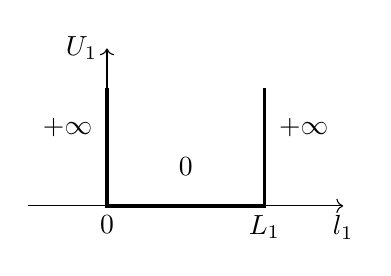
\begin{tikzpicture}
		\draw[->] (-1,0) -- (3,0) node[below] {$l_1$};
		\draw[->] (0,0) -- (0,2) node[left] {$U_1$};
		\draw[very thick] (0,1.5) -- (0,0) -- (2,0) -- (2,1.5);
		\node[below] at (0,0) {$0$};
		\node[below] at (2,0) {$L_1$};
		\node at (-0.5,1) {$+\infty$};
		\node at (1,0.5) {$0$};
		\node at (2.5,1) {$+\infty$};
	\end{tikzpicture}
	\quad
	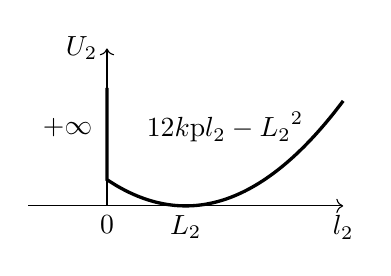
\begin{tikzpicture}
		\draw[->] (-1,0) -- (3,0) node[below] {$l_2$};
		\draw[->] (0,0) -- (0,2) node[left] {$U_2$};
		\draw[very thick] (0,1.5) -- plot[smooth,variable=\x,domain=0:3] ({\x},{(\x-1)^2/3});
		\node[below] at (0,0) {$0$};
		\node[below] at (1,0) {$L_2$};
		\node at (-0.5,1) {$+\infty$};
		\node at (1.5,1) {$\dfr12k\p{l_2-L_2}^2$};
	\end{tikzpicture}
	\quad
	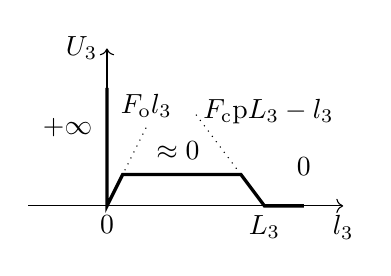
\begin{tikzpicture}
		\draw[->] (-1,0) -- (3,0) node[below] {$l_3$};
		\draw[->] (0,0) -- (0,2) node[left] {$U_3$};
		\draw[very thick] (0,1.5) -- (0,0) -- (0.2,0.4) -- (1.7,0.4) -- (2,0) -- (2.5,0);
		\node[below] at (0,0) {$0$};
		\node[below] at (2,0) {$L_3$};
		\node at (-0.5,1) {$+\infty$};
		\node at (0.9,0.7) {$\approx0$};
		\node at (2.5,0.5) {$0$};
		\draw[dotted] (0,0) -- (0.5,1) node[above] {$F_\mrm ol_3$};
		\draw[dotted] (2,0) -- (1.1,1.2) node[right] {$F_\mrm c\p{L_3-l_3}$};
	\end{tikzpicture}
	\caption{}
	\label{fig:2}
\end{figure}

\begin{figure}[h!]
	\centering
	\begin{tikzpicture}[xscale=0.4,yscale=0.3]
		\draw (-6,-3) -- (-6,3);
		\draw (-6,-2) -- node[midway,below] {1} (2,-2);
		\draw (2,-3) -- (2,1);
		\draw (2,-1) -- node[midway,above] {2} (6,-1);
		\draw (6,-3) -- (6,3);
		\draw (-2,0) -- node[midway,above] {3} (2,0);
		\draw (-2,-1) -- (-2,3);
		\draw (-6,1) -- node[midway,above] {2} (-2,1);
		\draw (-2,2) -- node[midway,above] {1} (6,2);
		\draw[->] (-9,0) -- (-6,0) node[midway,above] {$F$};
		\draw[->] (9,0) -- (6,0) node[midway,above] {$F$};
	\end{tikzpicture}
	\caption{}
	\label{fig:1}
\end{figure}

\mypara
将 $F$ 缓慢地从 $-\infty$ 变化至 $+\infty$.
定性描述 $l$ 在这期间的变化过程.

\mypara
将 $F$ 缓慢地从 $+\infty$ 变化至 $-\infty$.
定性描述 $l$ 在这期间的变化过程.

\newpage
\section{参考答案}

\subsection{喷流}

\mypara
设喷流的速度大小为 $\beta c$, 方向为 $\tht$.
在喷流运动了 $\Dlt t'$ 的时间前后各向地球发出一束光线. 如图~\ref{fig:jets} 所示.

\begin{figure}[h!]
	\centering
	\begin{tikzpicture}[scale=0.5]
		\begin{scope}[decoration={markings,mark=at position 0.5 with {\arrow{>}}}]
			\draw[postaction={decorate}] (-3,-2) node[left] {天体} -- node[midway,below right] {喷流} (0,0);
			\draw[postaction={decorate}] (0,0) -- (3,2);
			\draw[postaction={decorate}] (0,0) -- (10,0);
			\draw[postaction={decorate}] (3,2) -- node[midway,below] {光线} (10,2);
		\end{scope}
		\node at (10,1) {地球};
		\draw[|<->|] (-3,0) -- node[midway,left] {$\Dt y$} (-3,2);
		\draw[|<->|] (-0.2,0.3) -- node[midway, above left] {$\beta c\Dt t'$} ++(3,2);
		\node[above right,xshift=15] at (0,0) {$\tht$};
	\end{tikzpicture}
	\caption{}
	\label{fig:jets}
\end{figure}

两束光线到达地球的时间分别为 $D/c$ 和 $\Dt t'+\p{D-\beta c\Dt t'\cos\tht}/c$.
由此获得时间差
\[\Dt t=\Dt t'-\beta\Dt t'\cos\tht.\]
这两束光线的距离为 $\Dt y=\beta c\Dt t'\sin\tht$, 因此喷流的视速率为
\[\fr{\Dt y}{\Dt t}=\fr{\beta\sin\tht}{1-\beta\cos\tht}c.\]
对于锐角 $\tht$, 这是接近喷流. 对于远离喷流, 只需替换 $\tht\to\pi-\tht$ 即可.

因此可以获得两束喷流在天球上的角速度大小:
\[\mu_\mrm a=\fr1D\fr{\Dt y}{\Dt t}=\fr{\beta\sin\tht}{1-\beta\cos\tht}\fr cD,\quad
\mu_\mrm r=\fr{\beta\sin\tht}{1+\beta\cos\tht}\fr cD.\]
由此反解 $\beta,\tht$, 获得
\[\tan\tht=\fr{2D}c\fr{\mu_\mrm a\mu_\mrm r}{\mu_a-\mu_\mrm r},\quad
\beta\cos\tht=\fr{\mu_\mrm a-\mu_\mrm r}{\mu_\mrm a+\mu_\mrm r}.\]

\mypara
设进动角速度的方向为 $\vphi$, 其与自转轴的夹角为 $\psi$.
在进动的过程中, $\tht$ 的变化范围是 $\b{\v{\vphi-\psi},\vphi+\psi}$.
应用 Doppler 效应的公式时, 注意角度是观察者系中的, 于是得到
\[\lmd=\gma\p{1-\beta\cos\tht}\lmd_0,\]
其中 $\gma\ceq\p{1-\beta^2}^{-1/2}$.
因此,
\[\lmd_{\mrm a1,2}=\p{1-\beta\fc\cos{\vphi\mp\psi}}\gma\lmd_0,\quad
\lmd_{\mrm b1,2}=\p{1+\beta\fc\cos{\vphi\pm\psi}}\gma\lmd_0.\]
题中所说已知量的冗余可以看出指的是 $\lmd_{\mrm a2}+\lmd_{\mrm b1}=\lmd_{\mrm a1}+\lmd_{\mrm b2}$,
因此这里的 4 个方程只有 3 个独立.
由这些方程反解 $\beta,\vphi,\psi$, 可以解得
\[\vphi=\fr12\p{
	\arccos\fr{\lmd_{\mrm b1}-\lmd_{\mrm a2}}{\sqrt{\p{\lmd_{\mrm b1}+\lmd_{\mrm a2}}^2-4\lmd_0^2}}
	\pm\arccos\fr{\lmd_{\mrm b2}-\lmd_{\mrm a1}}{\sqrt{\p{\lmd_{\mrm b2}+\lmd_{\mrm a1}}^2-4\lmd_0^2}}
}.\]
式中 ``$\pm$'' 对应于两个物理上可能的解.
还可以加上 $\pi$ 的整数倍获得更多的解, 但最终只会有两个不同的锐角解.

\mypara
该问题涉及多个效应: 光行差, 宏观 Doppler 效应, 以及微观 Doppler 效应.
光行差指光的传播方向变化, 导致立体角变化;
宏观 Doppler 效应指的是先后到达地球的光线时间差不等于发出它们的时间差;
微观 Doppler 效应指的是光线的频率的变化, 导致每个光子的能量变化.
具体思路是, 将视光度表达为
\[S_\mrm{obs}\d t_\mrm{obs}=\int_\text{特定频率范围}\int_\text{光圈张成的立体角}
\fc{I_\mrm{obs}}{\nu,\Omg}\d\nu\d\Omg\d t_\mrm{obs},\]
其中 $I_\mrm{obs}\d\nu_\mrm{obs}$ 是观察者系中单位立体角的功率随频率的分布,
$\Omg$ 是 $\p{\tht,\vphi}$ 的缩写, $\d\Omg=\sin\tht\d\tht\d\vphi$.
这里需要注意的是, 积分范围是与参考系无关的
(因为 $S_\mrm{rest}$ 是在假设喷流与地球相对静止的情况下得到的),
所以实际上被积变量 $\nu,\Omg$ 可以任意替换名字,
比如说可以换成 $\nu_\mrm{rest},\Omg_\mrm{rest}$, 只需要保证积分范围和被积函数不变即可;
但是\tbf{不能}说 $\d\nu_\mrm{obs}=\d\nu_\mrm{rest}$.
然后, 研究光行差效应可获得 $\d\Omg_\mrm{obs}$ 与 $\d\Omg_\mrm{rest}$ 的关系;
研究宏观 Doppler 效应可获得 $\d t_\mrm{obs}$ 与 $\d t_\mrm{rest}$ 的关系;
研究微观 Doppler 效应可获得 $I_\mrm{obs}\d\Omg_\mrm{obs}\d t_\mrm{obs}$
与 $I_\mrm{rest}\d\Omg_\mrm{rest}\d t_\mrm{rest}$ 的关系.
利用 Lorentz 不变量 (光子数不变)
\[\fc{N_\mrm{obs}}{\nu_\mrm{obs},\Omg_\mrm{obs}}\d\nu_\mrm{obs}\d\Omg_\mrm{obs}\d t_\mrm{obs}
=\fc{N_\mrm{rest}}{\nu_\mrm{rest},\Omg_\mrm{rest}}\d\nu_\mrm{rest}\d\Omg_\mrm{rest}\d t_\mrm{rest}\]
即可最终获得 $S_\mrm{obs}$ 与 $S_\mrm{rest}$ 的关系,
其中 $N_\mrm{obs}\d\nu_\mrm{obs}$ 是单位立体角内单位时间发出的光子数随频率的分布.

首先考虑光行差. 利用速度合成公式, 可以容易得到,
对于在观察者系中出射角 (出射方向与运动方向的夹角) 为 $\tht_\mrm{obs}$ 的光线, 在静止系中其出射角为
\[\cos\tht_\mrm{rest}=\fr{\cos\tht_\mrm{obs}-\beta}{1-\beta\cos\tht_\mrm{obs}}.\]
于是, 可以计算得立体角 (注意 $\vphi_\mrm{obs}=\vphi_\mrm{rest}$)
\[\d\Omg_\mrm{rest}=\sin\tht_\mrm{rest}\d\tht_\mrm{rest}\d\vphi_\mrm{rest}
=\fr{\sin\tht_\mrm{obs}\d\tht_\mrm{obs}\d\vphi_\mrm{obs}}{\gma^2\p{1-\beta\cos\tht_\mrm{obs}}^2}
=\dlt^2\d\Omg_\mrm{obs},\]
其中 $\dlt\ceq\gma^{-1}\p{1-\beta\cos\tht_\mrm{obs}}^{-1}$ 是 Doppler 因子.

然后考虑宏观 Doppler 效应. \tbf{不能}由钟慢效应简单得到 $\d t_\mrm{obs}=\gma^{-1}\d t_\mrm{rest}$.
要理解这一点, 可以这么考虑: 光源每单位时间发射一定数量的光子, 这定义了一个频率 $f_\mrm{rest}$.
单位时间内, 观察者又会看到一定数量的光子, 这是另一个频率 $f_\mrm{obs}$.
这两个频率之间的关系 $f_\mrm{obs}=\dlt f_\mrm{rest}$ 就是 Doppler 效应.
而 $\d t_\mrm{rest}$ 的意义是, 静止系中发射一定数量
$f_\mrm{rest}\d t_\mrm{rest}$ 的光子所需要的总时间, 它会反比于这个频率.
所以得到 $\d t_\mrm{obs}=\dlt^{-1}\d t_\mrm{rest}$.

最后探讨微观 Doppler 效应.
我们知道
\[\fc{I_\mrm{rest}}{\nu,\Omg}\d\nu=h\nu\fc{N_\mrm{rest}}{\nu,\Omg}\d\nu,\quad
\fc{I_\mrm{obs}}{\nu,\Omg}\d\nu=h\nu\fc{N_\mrm{obs}}{\nu,\Omg}\d\nu,\]
其中 $h\nu$ 是频率为 $\nu$ 的单个光子的能量.
另一方面, 题目给出了 $\fc{I_\mrm{rest}}{\nu,\Omg}\propto\nu^\alp$, 于是可知
\[\fc{N_\mrm{rest}}{\nu,\Omg}=K\nu^{\alp-1},\]
其中 $K$ 是比例常数.
由 Doppler 效应知 $\nu_\mrm{obs}=\dlt\nu_\mrm{rest}$, 因此由光子数的 Lorentz 不变性可知
\begin{align*}
	\fc{N_\mrm{obs}}{\nu_\mrm{obs},\Omg_\mrm{obs}}\d\nu_\mrm{obs}\d\Omg_\mrm{obs}\d t_\mrm{obs}
	&=\fc{N_\mrm{rest}}{\nu_\mrm{rest},\Omg_\mrm{rest}}\d\nu_\mrm{rest}\d\Omg_\mrm{rest}\d t_\mrm{rest}\\
	&=K\nu_\mrm{rest}^{\alp-1}\d\nu_\mrm{rest}\d\Omg_\mrm{rest}\d t_\mrm{rest}\\
	&=\dlt^{-\alp}K\nu_\mrm{obs}^{\alp-1}\d\nu_\mrm{obs}\d\Omg_\mrm{rest}\d t_\mrm{rest}\\
	&=\dlt^{-\alp}\fc{N_\mrm{rest}}{\nu_\mrm{obs},\Omg_\mrm{obs}}\d\nu_\mrm{obs}\d\Omg_\mrm{rest}\d t_\mrm{rest}.
\end{align*}

综合三种效应, 可以得到
\begin{align*}
	\fc{I_\mrm{obs}}{\nu_\mrm{obs},\Omg_\mrm{obs}}\d\nu_\mrm{obs}\d\Omg_\mrm{obs}\d t_\mrm{obs}
	&=h\nu_\mrm{obs}\fc{N_\mrm{obs}}{\nu_\mrm{obs},\Omg_\mrm{obs}}\d\nu_\mrm{obs}\d\Omg_\mrm{obs}\d t_\mrm{obs}\\
	&=\dlt^{-\alp}h\nu_\mrm{obs}\fc{N_\mrm{rest}}{\nu_\mrm{obs},\Omg_\mrm{obs}}\d\nu_\mrm{obs}\d\Omg_\mrm{rest}\d t_\mrm{rest}\\
	&=\dlt^{-\alp}\fc{I_\mrm{rest}}{\nu_\mrm{obs},\Omg_\mrm{obs}}\d\nu_\mrm{obs}\,\dlt^2\d\Omg_\mrm{obs}\d t_\mrm{rest}.
\end{align*}
现在, 两边对 $\nu_\mrm{obs},\Omg_\mrm{obs}$ 积分, 然后除以 $\d t_\mrm{obs}$, 可得
\begin{align*}
	S_\mrm{obs}&=\fr1{\d t_\mrm{obs}}\int\fc{I_\mrm{obs}}{\nu,\Omg}\d\nu\d\Omg\d t_\mrm{obs}\\
	&=\dlt^{2-\alp}\fr1{\d t_\mrm{obs}}\int\fc{I_\mrm{rest}}{\nu,\Omg}\d\nu\d\Omg\d t_\mrm{rest}\\
	&=\dlt^{3-\alp}\fr1{\d t_\mrm{rest}}\int\fc{I_\mrm{rest}}{\nu,\Omg}\d\nu\d\Omg\d t_\mrm{rest}\\
	&=\dlt^{3-\alp}S_\mrm{rest}.
\end{align*}
这里 $S_\mrm{rest}$ 就是题目中所给的 $S_0$. 因此,
\[S_\mrm{obs}=\p{1-\beta^2}^{\p{3-\alp}/2}\p{1-\beta\cos\tht}^{\alp-3}S_0.\]

\tit{另}: 可利用结论: $I/\nu^3$ 是 Lorentz 不变量, 其中 $I\d\nu$ 是单位立体角的功率随频率的分布.
于是可以直接获得
\[I_\mrm{obs}=I_\mrm{rest}\p{\fr{\nu_\mrm{obs}}{\nu_\mrm{rest}}}^3
=\dlt^3I_\mrm{rest}=\dlt^3K\nu_\mrm{rest}^\alp=\dlt^{3-\alp}K\nu_\mrm{obs}^\alp.\]
获得跟上一种解法相同的结果 (因子 $\dlt^{3-\alp}$).

\subsection{轴子}

\subsection{缓慢拉伸}

为简洁起见, 选取单位使得 $k=1$.

由对称性可知, 虽然有两个装置 1 和两个装置 2,
但是两个装置 1 的长度相同, 两个装置 2 的长度也相同.
设三种装置的长度分别为 $l_1,l_2,l_3$,
三种装置上的压力分别为 $F_1,F_2,F_3$.
以下方程和不等式在任何情况下都成立:
\begin{gather*}
	l=l_1+l_2=2l_2+l_3=2l_1-l_3,\quad l_1=l_2+l_3,\\
	F=F_1+F_2=2F_1+F_3=2F_2-F_3,\quad F_2=F_1+F_3,\\
	l_1\ge0,\quad l_2\ge0,\quad l_3\ge0.
\end{gather*}
而如下三组条件中, 每一组内只有一个条件成立:
\begin{align*}
	&\left[\begin{aligned}
		&\mrm{1a}:\quad l_1<L_1,\quad F_1=0,\\
		&\mrm{1b}:\quad l_1=L_1,\quad F_1<0,
	\end{aligned}\right.\\
	&\left[\begin{aligned}
		&\mrm{2a}:\quad l_2=0,\quad F_2>L_2,\\
		&\mrm{2b}:\quad l_2>0,\quad F_2=L_2-l_2,\\
	\end{aligned}\right.\\
	&\left[\begin{aligned}
		&\mrm{\color{red}3a}:\quad l_3=0,\quad F_3>-F_\mrm o,\\
		&\mrm{\color{green!50!black}3d}:\quad 0<l_3<L_3,\quad F_3=0,\\
		&\mrm{\color{blue}3b}:\quad l_3=L_3,\quad 0<F_3<F_\mrm c,\\
		&\mrm{\color{blue}3c}:\quad l_3>L_3,\quad F_3=0.
	\end{aligned}\right.
\end{align*}
总共有 $2\cdot2\cdot4=16$ 种不同的组合.
对于每一种组合, 所有的条件给出了一个线性不等式系统,
可以系统性地用 Fourier--Motzkin 消元法求解出 $\p{l,F}$ 的取值范围,
也可以对每种情况用不等式操作来求解.
接下来考虑每一种情况.

对于情况 1a2a{\color{red}3a}, 有 $l_1=l_2=l_3=0$,
而 $F_1=0$, 以及 $F_2=F_3>L_2$.
因此,
\[\mrm{1a2a\color{red}3a}:\quad l=0,\quad F>L_2.\]

对于情况 1a2a{\color{blue}3b}, 有 $l_1=l_3=L_3$ 和 $l_2=0$.
另一方面, $F_1=0$, 而 $L_2<F_2=F_3<F_\mrm c$.
因此,
\[\mrm{1a2a\color{blue}3b}:\quad l=L_3,\quad L_2<F<F_\mrm c.\]

对于情况 1a2a{\color{blue}3c}
和情况 1a2a{\color{green!50!black}3d},
因为 $L_2<F_2=F_3=0$, 所以不可能发生.

对于情况 1a2b{\color{red}3a}, 有 $l_2=l_1<L_1$ 和 $l_3=0$.
另外, 有 $F_1=0$ 和 $L_2-l_2=F_2=F_3>-F_\mrm o$.
该不等式给出 $l_2<L_2+F_\mrm o$.
因此,
\[\mrm{1a2b\color{red}3a}:\quad
0<l<\opc{min}{2L_1,2\p{L_2+F_\mrm o}},\quad
F=L_2-\fr12l.\]

对于情况 1a2b{\color{blue}3b}, 有 $l_3=L_3$.
于是由 $l=2l_2+l_3=2l_1-l_3$ 得 $L_3<l<2L_1-L_3$.
另外, 有 $F_1=0$ 和 $0<L_2-l_2=F_2=F_3<F_\mrm c$.
代入 $l_2=\p{l-L_3}/2$ 可解得
$2L_2+L_3-2F_\mrm c<l<2L_2+L_3$.
因此,
\[\mrm{1a2b\color{blue}3b}:\quad
\opc{max}{L_3,2L_2+L_3-2F_\mrm c}<l<\opc{min}{2L_1-L_3,2L_2+L_3},\quad
F=L_2+\fr12L_3-\fr12l\quad\p{L_3<L_1}.\]

对于情况 1a2b{\color{blue}3c},
有 $F_1=F_2=F_3=0$, 因此 $F=0$.
此时有 $L_2=l_2=l_1-l_3<L_1-L_3$, 所以 $l=l_1+l_2<2L_1-L_3$.
另一方面, 有 $l=l_1+l_2<L_1+L_2$.
另外, 有 $l=2l_2+l_3>2L_2+L_3$.
因此,
\[\mrm{1a2b\color{blue}3c}:\quad
2L_2<l<\opc{min}{2L_1-L_3,L_1+L_2},\quad F=0\quad\p{L_3<L_1}.\]

对于情况 1a2b{\color{green!50!black}3d},
$F=0$ 和 $l<L_1+L_2$ 与上一种情况相同.
但是, 由 $l=2l_2+l_3$ 可知 $2L_2<l<2L_2+L_3$.
因此,
\[\mrm{1a2b\color{green!50!black}3d}:\quad
2L_2<l<\opc{min}{2L_2+L_3,L_1+L_2},\quad F=0.\]

对于情况 1b2a{\color{red}3a}, 有 $L_1=l_1=l_2+l_3=0$, 所以不可能出现.

对于情况 1b2a{\color{blue}3b}, 有 $L_1=l_1=l_2+l_3=L_3$.
因此, 这种情况只可能出现在 $L_3=L_1$ 时.
此时, $F=2F_1+F_3<F_\mrm c$,
而 $F=2F_2-F_3>2L_2-F_\mrm c$.
因此,
\[\mrm{1b2a\color{blue}3b}:\quad
l=L_1,\quad
2L_2-F_\mrm c<F<F_\mrm c\quad\p{L_3=L_1}.\]
可以发现, 其实这就是将 1a2a{\color{blue}3b} 和 1b2b{\color{blue}3b}
在 $L_3=L_1$ 时的情况合并在一起了,
所以以后可以不必考虑这种情况.

对于情况 1b2a{\color{blue}3c}
和情况 1b2a{\color{green!50!black}3d},
因为 $L_2<F_2=F_1<0$, 所以不可能出现.

对于情况 1b2b{\color{red}3a}, 有 $l_1=l_2=L_1$ 和 $l_3=0$.
另外, 有 $F_2=L_2-l_2=L_2-L_1$.
因此, $F=2F_2-F_3<2\p{L_2-L_1}+F_\mrm o$.
另一方面, $F=F_1+F_2<L_2-L_1$.
因此,
\[\mrm{1b2b\color{red}3a}:\quad
l=2L_1,\quad F<\opc{min}{L_2-L_1,2\p{L_2-L_1}+F_\mrm o}.\]

对于情况 1b2b{\color{blue}3b}, 有 $l_2=l_1-l_3=L_1-L_3$,
所以 $F_2=L_2-l_2=L_2-L_1+L_3$.
由 $F=2F_2-F_3$ 可知
$2\p{L_2-L_1+L_3}-F_\mrm c<F<2\p{L_2-L_1+L_3}$.
另外有 $F=F_1+F_2<L_2-L_1+L_3$.
因此,
\[\mrm{1b2b\color{blue}3b}:\quad
l=2L_1-L_3,\quad
2\p{L_2-L_1+L_3}-F_\mrm c<F<\opc{min}{2\p{L_2-L_1+L_3},L_2-L_1+L_3}
\quad\p{L_3<L_1}.\]

对于情况 1b2b{\color{blue}3c},
有 $l=2l_1-l_3<2L_1-L_3$,
以及 $F=2F_2-F_3=2\p{L_2-l+L_1}$.
由 $F=2F_1+F_3<0$ 解得 $l>L_1+L_2$.
因此,
\[\mrm{1b2b\color{blue}3c}:\quad
L_1+L_2<l<2L_1-L_3,\quad F=2\p{L_1+L_2-l},\quad
\p{L_3<L_1}.\]

对于情况 1b2b{\color{green!50!black}3d},
$F=2\p{L_1+L_2-l}$ 和 $l>L_1+L_2$ 与上一种情况相同.
但是, 由 $l=2l_1-l_3$ 得 $2L_1-L_3<l<2L_1$.
因此,
\[\mrm{1b2b\color{green!50!black}3d}:\quad
\opc{max}{2L_1-L_3,L_1+L_2}<l<2L_1,\quad
F=2\p{L_1+L_2-l}.\]

至此, 所有情况都已讨论完毕.
视 $L_{1,2,3},F_{\mrm o,\mrm c}$ 的大小关系不同,
$\p{l,F}$ 的图像会有定性上的不同,
且情况较为繁杂.
但是, 原则上, 在画出图像之后, 给出最终解答就很容易了.
只需要沿着图像上的线向上或者向下移动即可, 并且尽量不切换颜色.
在 $F=\pm\infty$ 时, 只有情况 1a2a{\color{red}3a} 和 1b2b{\color{red}3a} 会出现,
所以一开始一定是沿着红色的线移动.
若不得不切换颜色, 则尽量选择红色和蓝色的线, 其次选择绿色的线
(这是因为在装置 3 上有拉力或压力的情况下, 它的长度不会停留在 $0$ 到 $L_3$ 之间;
严格来说, 具体情况要取决于实际装置中的阻力, 外力变化的缓慢程度,
以及装置的惯性, 不过这不会影响定性结论).

\mypara
首先考虑所有的红线, 包括
1a2a{\color{red}3a}, 1a2b{\color{red}3a},
和 1b2b{\color{red}3a}.
对于 $L_2-L_1+F_\mrm o\gtrless0$ 两种情况,
它们的图像如图~\ref{fig:AFM} 所示.
图中标记的点的坐标分别为
\[\mrm A\p{2L_1,\opc{min}{L_2-L_1,2\p{L_2-L_1}+F_\mrm o}},\quad
\mrm F\p{2\opc{min}{L_1,L_2+F_\mrm o},\opc{max}{L_2-L_1,-F_\mrm o}},\quad
\mrm M\p{0,L_2}.\]
可以看到, 当 $L_2-L_1+F_\mrm o>0$ 时,
点 A 和 F 重合, 从而仅用红线即可连接 $F=-\infty$ 和 $F=+\infty$,
不需要切换颜色.
这种情况下, $l$ 的变化情况是先保持 $2L_1$ 不变, 然后线性减少至 $0$, 再保持不变.
此后, 我们只考虑 $L_2-L_1+F_\mrm o<0$ 的情况.

\begin{figure}[h!]
	\centering
	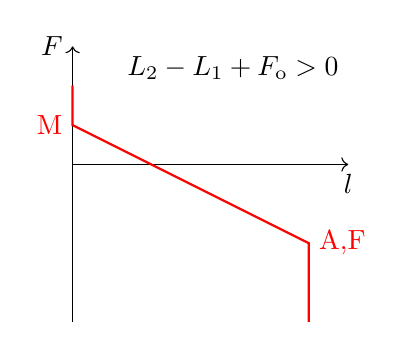
\begin{tikzpicture}[scale=0.5]
		\draw[->] (0,0) -- (7,0) node[below] {$l$};
		\draw[->] (0,-4) -- (0,3) node[left] {$F$};
		\draw[thick,red] (0,2) -- (0,1) node[left] {M}
			-- (6,-2) node[right] {A,F} -- (6,-4);
		\node[below left] at (7,3) {$L_2-L_1+F_\mrm o>0$};
	\end{tikzpicture}
	\quad
	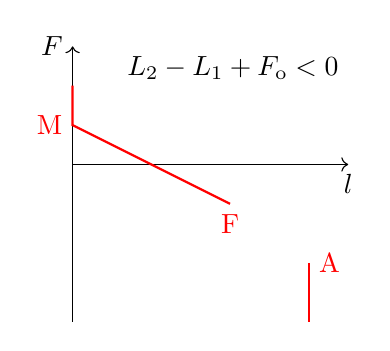
\begin{tikzpicture}[scale=0.5]
		\draw[->] (0,0) -- (7,0) node[below] {$l$};
		\draw[->] (0,-4) -- (0,3) node[left] {$F$};
		\draw[thick,red] (0,2) -- (0,1) node[left] {M}
			-- (4,-1) node[below] {F};
		\draw[thick,red] (6,-2.5) node[right] {A} -- (6,-4);
		\node[below left] at (7,3) {$L_2-L_1+F_\mrm o<0$};
	\end{tikzpicture}
	\caption{}
	\label{fig:AFM}
\end{figure}

在 $F=-\infty$ 时, 位于情况 1b2b{\color{red}3a}.
先考虑 1b2b{\color{red}3a}, 1b2b{\color{green!50!black}3d} 的一个端点 B,
和 1b2b{\color{blue}3b} 的一个端点 C.
对于 $2L_3-F_\mrm c\gtrless F_\mrm o$ 两种情况,
它们在图像上的样子如图~\ref{fig:ABC} 所示.
另外要注意 1b2b{\color{blue}3b} 只在 $L_3<L_1$ 时才存在.
图中标记的点的坐标为
\[\mrm B\p{2L_1,2\p{L_2-L_1}},\quad
\mrm C\p{2L_1-L_3,2\p{L_2-L_1+L_3}-F_\mrm c}.\]
因此, 我们可以发现, 在
$2L_3-F_\mrm c<F_\mrm o$ 且 $L_3<L_1$ 时, 动点 $\p{l,F}$
会在到达点 A 后切换到蓝线, 因此能观察到 $l$ 突然减小, 然后保持不变;
而在另一种情况 ($2L_3-F_\mrm c>F_\mrm o$ 或 $L_3>L_1$) 下,
它会在到达点 A 后切换到绿线,
因此能观察到 $l$ 突然减小, 然后线性减小.

\begin{figure}[h!]
	\centering
	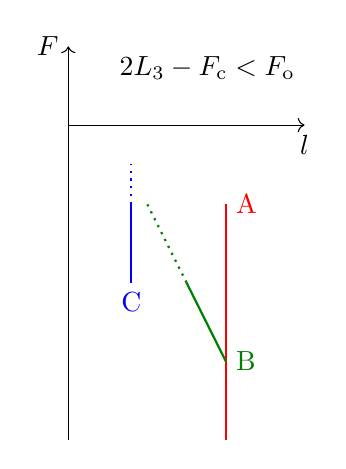
\begin{tikzpicture}
		\draw[->] (0,0) -- (3,0) node[below] {$l$};
		\draw[->] (0,-4) -- (0,1) node[left] {$F$};
		\draw[thick,red] (2,-1) node[right] {A} -- (2,-4);
		\draw[thick,green!50!black] (2,-3) node[right] {B} -- (1.5,-2);
		\draw[thick,green!50!black,dotted] (1.5,-2) -- (1,-1);
		\draw[thick,blue] (0.8,-2) node[below] {C} -- (0.8,-1);
		\draw[thick,blue,dotted] (0.8,-1) -- (0.8,-0.5);
		\node[below left] at (3,1) {$2L_3-F_\mrm c<F_\mrm o$};
	\end{tikzpicture}
	\quad
	\begin{tikzpicture}
		\draw[->] (0,0) -- (3,0) node[below] {$l$};
		\draw[->] (0,-4) -- (0,1) node[left] {$F$};
		\draw[thick,red] (2,-2) node[right] {A} -- (2,-4);
		\draw[thick,green!50!black] (2,-3) node[right] {B} -- (1.5,-2);
		\draw[thick,green!50!black,dotted] (1.5,-2) -- (1,-1);
		\draw[thick,blue] (0.8,-1.5) node[below] {C} -- (0.8,-1);
		\draw[thick,blue,dotted] (0.8,-1) -- (0.8,-0.5);
		\node[below left] at (3,1) {$2L_3-F_\mrm c>F_\mrm o$};
	\end{tikzpicture}
	\caption{}
	\label{fig:ABC}
\end{figure}

接下来考虑 1b2b{\color{green!50!black}3d} (BD),
1b2b{\color{blue}3b} (CE),
3b2b{\color{blue}3c} (EH),
1a2b{\color{blue}3c} (HG),
1a2b{\color{blue}3b} 的一个端点 G,
以及 1a2b{\color{green!50!black}3d} (JI).
对于 $L_2-L_1+L_3\gtrless0$ 两种情况,
它们在图像上的样子如图~\ref{fig:CEHG} 所示.
另外要注意, 对于 $L_2-L_1+L_3>0$ 的情况,
还要考虑到图中的蓝线只在 $L_3<L_1$ 时存在.
图中标记的点的坐标为
\begin{gather*}
	\mrm D\p{\opc{max}{L_1+L_2,2L_1-L_3},\opc{min}{2\p{L_2-L_1+L_3},0}},\quad
	\mrm E\p{2L_1-L_3,\opc{min}{2\p{L_2-L_1+L_3},L_2-L_1+L_3}},\\
	\mrm G\p{\opc{min}{2L_1-L_3,2L_2+L_3},\opc{max}{L_2-L_1+L_3,0}},\quad
	\mrm H\p{\opc{min}{2L_1-L_3,L_1+L_2},\opc{max}{L_2-L_1+L_3,0}},\\
	\mrm I\p{2L_2,0},\quad
	\mrm J\p{\opc{min}{L_1+L_2,2L_2+L_3},0}.
\end{gather*}
如果上一步中, 动点 $\p{l,F}$ 沿着蓝线 CE 向上移动,
那么会有两种情况:
若 $L_2-L_1+L_3<0$, 则 $l$ 会在保持不变后, 线性减小,
然后再突然减小, 然后再线性减小;
若 $L_2-L_1+L_3>0$, 则 $l$ 会在保持不变后, 线性减小.
如果上一步中, 动点 $\p{l,F}$ 沿着绿线 BD 向上移动,
那么会有两种情况:
若 $L_2-L_1+L_3<0$, 则 $l$ 会在线性减小后, 切换到蓝线并继续线性减小,
然后突然减小, 再继续线性减小;
若 $L_2-L_1+L_3>0$
(如果 $L_3<L_1$, 那么一定会处于这种情况;
这种情况不涉及蓝线, 所以仍然成立), 则 $l$ 会在线性减小后, 突然减小.

\begin{figure}[h!]
	\centering
	\begin{tikzpicture}
		\draw[->] (0,0) -- (5,0) node[below] {$l$};
		\draw[->] (0,-4) -- (0,2) node[left] {$F$};
		\draw[thick,green!50!black] (4.5,-3) node[right] {B}
			-- (4,-2) node[above right] {D\color{black},\color{blue}E};
		\draw[thick,blue] (4,-3.5) node[left] {C}
			-- (4,-2)
			-- (3,0) node[above] {H}
			-- (2,0) node[below] {G\color{black},\color{green!50!black}J} -- (1,0.5);
		\draw[thick,blue,dotted] (1,0.5) -- (0.5,0.75);
		\draw[thick,green!50!black] (2,0)
			-- (1,0) node[below] {I};
		\node[below left] at (5,2) {$L_2-L_1+L_3<0$};
	\end{tikzpicture}
	\quad
	\begin{tikzpicture}
		\draw[->] (0,0) -- (5,0) node[below] {$l$};
		\draw[->] (0,-4) -- (0,2) node[left] {$F$};
		\draw[thick,green!50!black] (5,-2) node[right] {B}
			-- (4,0) node[above] {D,J}
			-- (2,0) node[below] {I};
		\draw[thick,blue] (3,-3) node[left] {C}
			-- (3,0.5) node[above right] {E,H,G} -- (2,1);
		\draw[thick,blue,dotted] (2,1) -- (1,1.5);
		\node[below left] at (5,2) {$L_2-L_1+L_3>0$};
	\end{tikzpicture}
	\caption{}
	\label{fig:CEHG}
\end{figure}

接下来考虑 1a2b{\color{blue}3b} 的另一个端点 K,
1a2a{\color{blue}3b} (KL),
1a2b{\color{green!50!black}3d} (JI),
1a2b{\color{red}3a} (FM),
以及 1a2a{\color{red}3a} (M 到无穷远).
对于 $L_2\gtrless F_\mrm c$ 两种情况,
它们在图像上的样子如图~\ref{fig:KL} 所示.
注意 $L_3>L_1$ 时蓝线不存在,
但是此时动点 $\p{l,F}$ 的运动一定与蓝线无关了, 所以无需特别考虑.
图中标记的点的坐标为
\[\mrm K\p{\opc{max}{L_3,L_3+2\p{L_2-F_\mrm c}},\opc{min}{L_2,F_\mrm c}},\quad
\mrm L\p{\opc{max}{L_3,L_3+2\p{L_2-F_\mrm c}},F_\mrm c}.\]
如果上一步中, 动点 $\p{l,F}$ 沿着绿线 JI 向左移动,
那么在 $l$ 突然减小后, 会线性减小 (沿着红线 IM),
减小到 $0$ 后再保持不变.
如果在上一步中, 动点 $\p{l,F}$ 沿着蓝线 GK 移动,
那么会有两种情况:
若 $L_2<F_\mrm c$, 则 $l$ 会在线性减小之后,
保持不变, 然后再突然减小到 $0$ (切换到红色), 再继续保持不变;
若 $L_2>F_\mrm c$, 则 $l$ 会在线性减小之后,
突然减小 (切换到红色), 然后线性减小到 $0$,
再保持不变.

\begin{figure}[h!]
	\centering
	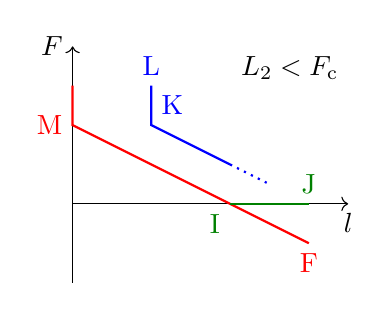
\begin{tikzpicture}
		\draw[->] (0,0) -- (3.5,0) node[below] {$l$};
		\draw[->] (0,-1) -- (0,2) node[left] {$F$};
		\draw[thick,red] (0,1.5)
			-- (0,1) node[left] {M}
			-- (3,-0.5) node[below] {F};
		\draw[thick,green!50!black] (2,0) node[below left] {I}
			-- (3,0) node[above] {J};
		\draw[thick,blue] (1,1.5) node[above] {L}
			-- (1,1) node[above right] {K} -- (2,0.5);
		\draw[thick,blue,dotted] (2,0.5) -- (2.5,0.25);
		\node[below left] at (3.5,2) {$L_2<F_\mrm c$};
	\end{tikzpicture}
	\quad
	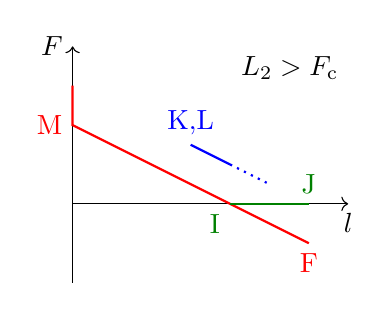
\begin{tikzpicture}
		\draw[->] (0,0) -- (3.5,0) node[below] {$l$};
		\draw[->] (0,-1) -- (0,2) node[left] {$F$};
		\draw[thick,red] (0,1.5)
			-- (0,1) node[left] {M}
			-- (3,-0.5) node[below] {F};
		\draw[thick,green!50!black] (2,0) node[below left] {I}
			-- (3,0) node[above] {J};
		\draw[thick,blue] (1.5,0.75) node[above] {K,L} -- (2,0.5);
		\draw[thick,blue,dotted] (2,0.5) -- (2.5,0.25);
		\node[below left] at (3.5,2) {$L_2>F_\mrm c$};
	\end{tikzpicture}
	\caption{}
	\label{fig:KL}
\end{figure}

至此 $F$ 已经到达 $+\infty$.
整个过程中 $l$ 的变化的定性描述由图~\ref{fig:compress} 中的流程图给出.

\begin{figure}[h!]
	\centering
	\begin{tikzpicture}[
		on grid,
		node distance=1.5cm and 4cm,
		startstop/.style = {
			rectangle,rounded corners,
			draw=black,
			text centered
		},
		process/.style = {
			rectangle,
			text centered,
			draw=black
		},
		decision/.style = {
			rectangle,
			text centered
		}
	]
		\node[startstop] (start) {开始};
		\node[process, left=of start] (red no change) {\color{red}不变};
		\node[decision, below=of red no change] (L2-L1+Fo) {$L_2-L_1+F_\mrm o<0$};
		\node[process, below=of L2-L1+Fo] (sudden 1) {突然减小};
		\node[decision, below=of sudden 1] (2L2-Fc-Fo) {$2L_3-F_\mrm c<F_\mrm o$ 且 $L_3<L_1$};
		\node[process, below=of 2L2-Fc-Fo] (blue no change 1) {\color{blue}不变};
		\node[process, right=of 2L2-Fc-Fo] (green dec) {\color{green!50!black}线性减小};
		\node[decision, below=of green dec] (L2-L1+L3 2) {$L_2-L_1+L_3<0$};
		\node[process, right=of L2-L1+L3 2] (green sudden) {\color{green!50!black}突然减小};
		\node[decision, below=of blue no change 1] (L2-L1+L3 1) {$L_2-L_1+L_3>0$};
		\node[process, right=of L2-L1+L3 1] (blue dec 1) {\color{blue}线性减小};
		\node[process, below=of L2-L1+L3 1] (blue dec 2) {\color{blue}线性减小};
		\node[process, right=of blue dec 2] (blue sudden) {\color{blue}突然减小};
		\node[decision, below=of blue dec 2] (L2-Fc) {$L_2<F_\mrm c$};
		\node[process, right=of L2-Fc] (sudden 2) {突然减小};
		\node[process, below=of L2-Fc] (blue no change 2) {\color{blue}不变};
		\node[process, right=of sudden 2] (red dec) {\color{red}线性减小};
		\node[process, right=of blue no change 2] (sudden 3) {突然减小};
		\node[process, below=of red dec] (red no change 2) {\color{red}不变};
		\node[startstop, right=of red no change 2] (stop) {结束};
		\draw[->] (start) -- (red no change);
		\draw[->] (red no change) -- (L2-L1+Fo);
		\draw[->] (L2-L1+Fo) -- node[left] {是} (sudden 1);
		\draw[->] (sudden 1) -- (2L2-Fc-Fo);
		\draw[->] (2L2-Fc-Fo) -- node[left] {是} (blue no change 1);
		\draw[->] (2L2-Fc-Fo) -- node[above] {否} (green dec);
		\draw[->] (blue no change 1) -- (L2-L1+L3 1);
		\draw[->] (green dec) -- (L2-L1+L3 2);
		\draw[->] (L2-L1+L3 2) -- node[above] {否} (green sudden);
		\draw[->] (L2-L1+L3 2) -- node[left] {是} (blue dec 1);
		\draw[->] (L2-L1+L3 1) -- node[above] {否} (blue dec 1);
		\draw[->] (blue dec 1) -- (blue sudden);
		\draw[->] (L2-L1+L3 1) -- node[left] {是} (blue dec 2);
		\draw[->] (blue sudden) -- (blue dec 2);
		\draw[->] (blue dec 2) -- (L2-Fc);
		\draw[->] (L2-Fc) -- node[left] {是} (blue no change 2);
		\draw[->] (L2-Fc) -- node[above] {否} (sudden 2);
		\draw[->] (blue no change 2) -- (sudden 3);
		\draw[->] (sudden 2) -- (red dec);
		\draw[->] (sudden 3) -- (red no change 2);
		\draw[->] (red dec) -- (red no change 2);
		\draw[->] (red no change 2) -- (stop);
		\draw[->] (green sudden) -- (red dec);
		\draw[->] (L2-L1+Fo) -- node[above] {否} ++(10cm,0cm) |- (red dec);
	\end{tikzpicture}
	\caption{}
	\label{fig:compress}
\end{figure}

\mypara
当 $F=+\infty$ 时, 装置处于 1a2a{\color{red}3a}.
当 $F$ 逐渐减小时, 点 $\p{l,F}$ 一点先沿着红线向下移动,
然后沿着红线 MF 移动直到点 F.
此时, 若 $L_2-L_1+F_\mrm o<0$, 它可以直接继续沿着红线向下移动到无穷远, 整个过程结束;
若 $L_2-L_1+F_\mrm o>0$, 则它会从点 F 横向突变,
而突变至蓝线还是绿线, 以及突变时 $l$ 会变大还是变小, 则取决于不同情况.

首先研究它会突变至蓝线还是绿线.
可以发现, 这取决于 F 的纵坐标和 C 纵坐标的大小关系.
如果 F 的纵坐标大于 C 的纵坐标 (即 $-F_\mrm o>2\p{L_2-L_1+L_3}-F_\mrm c$)
且 $L_3<L_1$,
则突变至蓝线, 否则突变至绿线.

当它突变至蓝线时, 又有两种情况:
如果 F 的纵坐标大于 E 的纵坐标
(即 $-F_\mrm o>2\p{L_2-L_1+L_3}$), 则突变至线段 HE, 否则突变至线段 EC.
如果 F 在线段 HE 的左侧
(即 $-F_\mrm o<2\p{L_1-L_2-2F_\mrm o}$)
或者在线段 EC 的左侧
(即 $2\p{L_2+F_\mrm o}<2L_1-L_3$), 那么突变时 $l$ 会增大,
否则突变时 $l$ 会减小.

当它突变至绿线时, 如果 F 在线段 BD 的左侧
(即 $-F_\mrm o<2\p{L_1-L_2-2F_\mrm o}$),
则突变时 $l$ 会增大,
否则突变时 $l$ 会减小.

\tit{注}: 可以看到, 对于某些情况, 在缓慢拉伸的过程中,
装置的长度反而会突然减小.
这个看似反直觉的现象被称为 Braess 悖论.

另外要注意, 对于突变到蓝线的情况, 如果 $2L_3-F_\mrm c>F_\mrm o$,
那么点 $\p{l,F}$ 在到达点 C 后无法直接突变到红线,
所以它会先突变到绿线, 最后再到达红线.

全过程的定性描述由图~\ref{fig:stretch} 中的流程图给出.

\begin{figure}[h!]
	\centering
	\begin{tikzpicture}[
		on grid,
		node distance=1.5cm and 4cm,
		startstop/.style = {
			rectangle,rounded corners,
			draw=black,
			text centered
		},
		process/.style = {
			rectangle,
			text centered,
			draw=black
		},
		decision/.style = {
			rectangle,
			text centered
		}
	]
		\node[startstop] (start) {开始};
		\node[process, left=of start] (red no change 1) {\color{red}不变};
		\node[process, left=of red no change 1] (red inc) {\color{red}线性增大};
		\node[decision, below=of red inc] (L2-L1+Fo) {$L_2-L_1+F_\mrm o<0$};
		\node[decision, below=of L2-L1+Fo] (Fc-Fo) {$F_\mrm o-F_\mrm c<2\p{L_1-L_2-L_3}$ 且 $L_3<L_1$};
		\node[decision, below=of Fc-Fo] (Fo 1) {$F_\mrm o<2\p{L_1-L_2-L_3}$};
		\node[decision, below=of Fo 1] (Fo 2) {$3F_\mrm o<2\p{L_1-L_2}$};
		\node[process, right=of Fo 2] (sudden dec HE) {突然减小};
		\node[process, below=of Fo 2] (sudden inc HE) {突然增大};
		\node[process, right=of sudden inc HE] (blue inc) {\color{blue}线性增大};
		\node[decision, below=of sudden inc HE] (Fo 3) {$2F_\mrm o<2\p{L_1-L_2}-L_3$};
		\node[process, right=of Fo 3] (sudden dec EC) {突然减小};
		\node[process, below=of Fo 3] (sudden inc EC) {突然增大};
		\node[process, right=of sudden inc EC] (blue no change) {\color{blue}不变};
		\node[process, below=of blue no change] (sudden inc) {突然增大};
		\node[decision, below=of sudden inc] (Fo 4) {$F_\mrm o>2L_3-F_\mrm c$};
		\node[process, left=of Fo 4] (green inc) {\color{green!50!black}线性增大};
		\node[process, above=of green inc] (sudden dec DB) {突然减小};
		\node[decision, left=of sudden dec DB] (Fo 5) {$3F_\mrm o<2\p{L_1-L_2}$};
		\node[process, below=of Fo 5] (sudden inc DB) {突然增大};
		\node[process, below=of Fo 4] (red no change 2) {\color{red}不变};
		\node[startstop, below=of red no change 2] (stop) {结束};
		\draw[->] (start) -- (red no change 1);
		\draw[->] (red no change 1) -- (red inc);
		\draw[->] (red inc) -- (L2-L1+Fo);
		\draw[->] (L2-L1+Fo) -- node[left] {是} (Fc-Fo);
		\draw[->] (Fc-Fo) -- node[right] {是} (Fo 1);
		\draw[->] (Fo 1) -- node[right] {是} (Fo 2);
		\draw[->] (Fo 2) -- node[left] {是} (sudden inc HE);
		\draw[->] (Fo 2) -- node[above] {否} (sudden dec HE);
		\draw[->] (sudden inc HE) -- (blue inc);
		\draw[->] (sudden dec HE) -- (blue inc);
		\draw[->] (Fo 3) -- node[left] {是} (sudden inc EC);
		\draw[->] (Fo 3) -- node[above] {否} (sudden dec EC);
		\draw[->] (sudden inc EC) -- (blue no change);
		\draw[->] (sudden dec EC) -- (blue no change);
		\draw[->] (blue no change) -- (sudden inc);
		\draw[->] (sudden inc) -- (Fo 4);
		\draw[->] (Fo 4) -- node[right] {是} (red no change 2);
		\draw[->] (Fo 4) -- node[above] {否} (green inc);
		\draw[->] (Fo 5) -- node[left] {是} (sudden inc DB);
		\draw[->] (Fo 5) -- node[above] {否} (sudden dec DB);
		\draw[->] (sudden inc DB) -- (green inc);
		\draw[->] (sudden dec DB) -- (green inc);
		\draw[->] (green inc) |- (red no change 2);
		\draw[->] (red no change 2) -- (stop);
		\draw[->] (L2-L1+Fo) -- node[above] {否} ++(7cm,0cm) |- (red no change 2);
		\draw[->] (Fc-Fo) -- node[above] {否} ++(-4cm,0cm) -- (Fo 5);
		\draw[->] (Fo 1) -- node[above] {否} ++(-3cm,0cm) |- (Fo 3);
		\draw[->] (blue inc) -- ++(2cm,0cm) |- (blue no change);
	\end{tikzpicture}
	\caption{}
	\label{fig:stretch}
\end{figure}

\end{document}
